\documentclass{article}
\usepackage{amsmath}
\usepackage{mathtools}
\usepackage{gensymb}
\usepackage[a4paper,inner=1.5cm,outer=1.5cm,top=2cm,bottom=0.5cm]{geometry} 
\usepackage{xcolor}                    
\usepackage{tikz}                           
\usepackage{multicol}
\usepackage{hyperref}
\usepackage{pgfplots}
\usetikzlibrary{calc}
\usetikzlibrary{intersections}
\usetikzlibrary{intersections,calc,angles,quotes}
\usetikzlibrary{shapes,arrows,positioning,decorations.pathreplacing,calc}
\usetikzlibrary{calc,angles,positioning,intersections,quotes,decorations.markings}
\usepackage{tkz-euclide}
\usetikzlibrary{backgrounds}
\usetikzlibrary{calc,through}
\usetikzlibrary{angles}
\usetikzlibrary{fadings}
\usetikzlibrary{shapes.geometric}
\usetikzlibrary{shapes.symbols}
\usepackage{draftwatermark}
\usepackage{mathptmx}

\SetWatermarkText{\textcolor{black!20}{Mathema Shukur}}
\SetWatermarkFontSize{2 cm}
\usepackage[utf8]{inputenc}
\usepackage{fontspec}

\setmainfont{[Kalpurush.ttf]}
\newfontface{\en}{[Arial.ttf]} %%this is optional, if you want to use a secondary font. Any english font is supported
\newlength\Radius
\setlength\Radius{4cm}
\begin{document} 
	\Large
	\textcolor{red}{Welcome To} 
	\\
	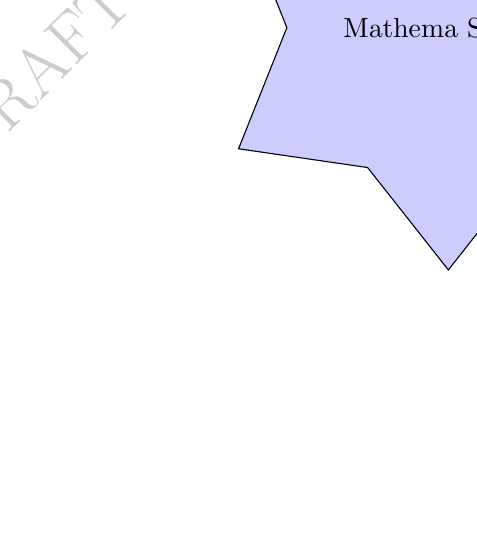
\begin{tikzpicture}
		\tikz \node [fill=blue!20,star,star points=6,draw] {Mathema Shukur };
	\end{tikzpicture}
	\\
	যাদের জন্যে প্রযোজ্যঃ  	\textcolor{magenta}{একাদশ ও দ্বাদশ শ্রেণীর শিক্ষার্থী} \\
	বিষয়ঃ \textcolor{magenta}{উচ্চতর গণিত ১ম পত্র} \\
	অধ্যায়ঃ \textcolor{magenta}{৪-বৃত্ত}\\ 
	\\
	\\
	\href{https://www.youtube.com/watch?v=DRxNte3mU6U&list=PLIjPH8h-K22w5iYZogyV1AI8-baSpY2Qn&index=1}{\textcolor{blue}{মূল বিন্দুতে (0,0) কেন্দ্র থাকলে বৃত্তের সমীকরণ কী?}}\\
	\\
	\href{https://www.youtube.com/watch?v=rGCA1MltZsY&list=PLIjPH8h-K22w5iYZogyV1AI8-baSpY2Qn&index=2}{\textcolor{blue}{কী শর্তে কেন্দ্রের স্থানাঙ্ক হতে বৃত্তের ব্যাসার্ধ নির্ণয় করা হয়?}}\\
	\\
	\href{https://www.youtube.com/watch?v=gehIW-_0XrQ&list=PLIjPH8h-K22w5iYZogyV1AI8-baSpY2Qn&index=3}{\textcolor{blue}{বৃত্তের সাধারণ সমীকরণ $x^2+y^2+2gx+2fy+c=0$}}\\
	\\
	\href{https://www.youtube.com/watch?v=WzuG-MuA6Cs&list=PLIjPH8h-K22w5iYZogyV1AI8-baSpY2Qn&index=4}{\textcolor{blue}{পোলার স্থানাঙ্কে বৃত্তের সমীকরণ নির্ণয়}}\\
	\\
	\href{https://www.youtube.com/watch?v=ssCuBx7HEHI&list=PLIjPH8h-K22w5iYZogyV1AI8-baSpY2Qn&index=5}{\textcolor{blue}{ব্যাসের প্রান্ত বিন্দু (x1,y1) ও (x2,y2) হলে বৃত্তের সমীকরণ নির্ণয়}}\\
	\\
	\href{https://www.youtube.com/watch?v=afVjGQrIpDs&list=PLIjPH8h-K22w5iYZogyV1AI8-baSpY2Qn&index=6}{\textcolor{blue}{বৃত্ত ও সরলরেখার ছেদবিন্দুগামী বৃত্তের সমীকরণ}}\\
	\\
	\href{https://www.youtube.com/watch?v=rXOyjYE6YfU&list=PLIjPH8h-K22w5iYZogyV1AI8-baSpY2Qn&index=7}{\textcolor{blue}{দুইটি বৃত্তকে ছেদ করে এমন বৃত্তের সমীকরণ}}\\
	\\
	\href{https://www.youtube.com/watch?v=iQIWTRqZsAY}{\textcolor{blue}{৩ টি বিন্দুগামী বৃত্তের সমীকরণ নির্ণয়}}\\
	\\
	\href{https://www.youtube.com/watch?v=zsiv_hlMIR0}{\textcolor{blue}{২ টি বৃত্ত পরস্পরকে স্পর্শ করার শর্ত}}\\
	\\
	(1a) $(x_1,y_1)$ বিন্দুতে   $x^2+y^2=a^2$  বৃত্তে অঙ্কিত স্পর্শকের সমীকরণ \\
	$xx_1+yy_1=a^2$\\
	\\ 
	(1b) $(x_1,y_1)$ বিন্দুতে  $x^2+y^2+2gx+2fy+c=0$  বৃত্তে অঙ্কিত স্পর্শকের সমীকরণ \\   $xx_1+yy_1+g(x+x_1)+f(y+y_1)+c=0$\\
	\\ 
	(2a) $(x_1,y_1)$ বিন্দুতে   $x^2+y^2=a^2$  বৃত্তে অঙ্কিত অভিলম্বের  সমীকরণ \\
	$x_1y-xy_1=0$\\
	\\ 
	(2b) $(x_1,y_1)$ বিন্দুতে  $x^2+y^2+2gx+2fy+c=0$  বৃত্তে অঙ্কিত অভিলম্বের সমীকরণ \\   $(x_1+g)y-(y_1+f)x+fx_1-gy_1=0$\\
	
	\textcolor{magenta}{[চট্রগ্রাম বোর্ড-২০১৪]}\\ 
	(1) $(4,-11)$ বিন্দুতে  $x^2+y^2-3x+10y=15$ বৃত্তের স্পর্শকের সমীকরণ নির্ণয় কর। \\ 
	\begin{align*}
		x^2+y^2-3x+10y&=15\\
		\\
		x^2+y^2+2\left(-\frac{3}{2}\right)x+2(5)y+(-15)&=0\\
		\boxed{\textcolor{blue}{x^2+y^2+2gx+2fy+c=0}}&\\
		g=\left(-\frac{3}{2}\right),\,\,&f=5,\,\,c=-15
	\end{align*}
	\\
	$x_1=4$,\,\,$y_1=-11$\\
	\\
	\begin{align*}
		xx_1+yy_1+g(x+x_1)+f(y+y_1)+c&=0\\
		\\
		x(4)+y(-11)+\left(-\frac{3}{2}\right)(x+4)+5(y-11)-15&=0\\
		\\
		4x-11y-\frac{3x}{2}-6+5y-55-15&=0\\
		\\
		8x-22y-3x-12+10y-110-30&=0\\
		\\
		5x-12y-152&=0\\
	\end{align*}
	\\
	\begin{tikzpicture}[transform shape,scale=1]
		\draw[thick,green] (1.5,-5) circle (6.5);
		\fill[green] (1.5,-5) circle (1 mm);
		\fill[green] (4,-11) circle (1 mm);
		\draw[magenta](-0.8,-13)--(7.6,-9.5);
			\node at (4,-11.5) {$\textcolor{green}{(4,-11)}$};
	\end{tikzpicture}\\
	\\ 
	\textcolor{magenta}{[ময়মনসিংহ বোর্ড-২০২২]}\\ 
(2)	$(-2,1)$ বিন্দুতে  $x^2+y^2-4x-6y-7=0$ বৃত্তের স্পর্শকের সমীকরণ নির্ণয় কর। \\ 
	\\
	\begin{align*}
		x^2+y^2-4x-6y-7&=0\\
		\\
		x^2+y^2+2(-2)x+2(-3)y+(-7)&=0\\
		\boxed{\textcolor{blue}{x^2+y^2+2gx+2fy+c=0}}&\\
		g=-2,\,\,&f=-3,\,\,c=-7
	\end{align*}
	\\
	$x_1=-2$,\,\,$y_1=1$\\
	\\
	\begin{align*}
		xx_1+yy_1+g(x+x_1)+f(y+y_1)+c&=0\\
		\\
		x(-2)+y(1)+(-2)(x-2)+(-3)(y+1)-7&=0\\
		\\
		-2x+y-2x+4-3y-3-7&=0\\
		\\
		-4x-2y-6&=0\\
		\\
		2x+y+3&=0 
	\end{align*}
	\\ 
	\begin{tikzpicture}[transform shape,scale=1]
		\draw[thick,green] (2,3) circle (4.47);
		\fill[green] (2,3) circle (1 mm);
		\fill[green] (-2,1) circle (1 mm);
		\draw[magenta](-5,7)--(0,-3);
			\node at (-3,1) {$\textcolor{green}{(-2,1)}$};
	\end{tikzpicture}\\
	\\ 
		\textcolor{magenta}{[যশোর  বোর্ড-২০১৬]}\\
(3)	$x^2+y^2=13$ বৃত্তের $(3,2)$ বিন্দুতে অভিলম্বের সমীকরণ নির্ণয় কর । \\
	\\
	\textcolor{blue}{	(2a) $(x_1,y_1)$ বিন্দুতে   $x^2+y^2=a^2$  বৃত্তে অঙ্কিত অভিলম্বের  সমীকরণ \\
		$x_1y-xy_1=0$\\}
	\\
	$3y-2x=0$\\
	\begin{tikzpicture}[transform shape,scale=1]
	\draw[thick,green] (0,0) circle (3.60);
	\fill[green] (0,0) circle (1 mm);
	\fill[green] (3,2) circle (1 mm);
	\draw[magenta](3,2)--(6,4);
	\node at (2.2,2) {$\textcolor{green}{(3,2)}$};
\end{tikzpicture}\\
\\ 

	\textcolor{magenta}{[দিনাজপুর  বোর্ড-২০১১]}\\
(4)	$x^2+y^2=20$ বৃত্তের  $2$ ভূজ বিশিষ্ট বিন্দুতে স্পর্শকের সমীকরণ নির্ণয় কর।\\
	বিন্দুটির ভুজ $x=2$\\
	\\
	\begin{align*}
		x^2+y^2&=20\\
		\\
		2^2+y^2&=20\\
		\\
		y^2&=20-4\\
		\\
		y^2&=16\\
		\\
		y&=\pm 4
	\end{align*}
	\\
	স্পর্শ বিন্দুগুলি $(2,4)$, \,\,$(2,-4)$\\
	\\
	\textcolor{blue}{(1a) $(x_1,y_1)$ বিন্দুতে   $x^2+y^2=a^2$  বৃত্তে অঙ্কিত স্পর্শকের সমীকরণ \\
		$xx_1+yy_1=a^2$\\}	
	\\
	$(2,4)$ বিন্দুতে স্পর্শকের সমীকরণ\\ 
	$2x+4y=20$\\
	$\Rightarrow x+2y=10$\\
	\\
	$(2,-4)$ বিন্দুতে স্পর্শকের সমীকরণ\\
	$2x-4y=20$\\
	$\Rightarrow x-2y=10$\\
	\begin{tikzpicture}[transform shape,scale=1]
	\draw[thick,green] (0,0) circle (4.47);
	\fill[green] (0,0) circle (1 mm);
	\fill[green] (2,-4) circle (1 mm);
	\fill[green] (2,4) circle (1 mm);
	\draw[magenta](10,0)--(0,5);
		\draw[magenta](10,0)--(0,-5);
	\node at (2,-4.5) {$\textcolor{green}{(2,-4)}$};
	\node at (2,4.5) {$\textcolor{green}{(2,4)}$};
\end{tikzpicture}\\
\\
	\textcolor{magenta}{[কুমিল্লা বোর্ড-২০০৫]}\\
(5) $x^2+y^2+4x-10y+28=0$ বৃত্তের  $(-2,4)$ বিন্দুতে স্পর্শক ও অভিলম্বের সমীকরণ নির্ণয় কর। \\
	\\
\begin{align*}
x^2+y^2+4x-10y+28&=0\\
	\boxed{\textcolor{blue}{x^2+y^2+2gx+2fy+c=0}}&\\
	x^2+y^2+2(2)x+2(-5)y+(28)&=0\\
	\\
	g=2,\,\,f=-5,\,\,c=28&
\end{align*}
\\
\textcolor{blue}{(1b) $(x_1,y_1)$ বিন্দুতে  $x^2+y^2+2gx+2fy+c=0$  বৃত্তে অঙ্কিত স্পর্শকের সমীকরণ \\   $xx_1+yy_1+g(x+x_1)+f(y+y_1)+c=0$\\ }
\\
\begin{align*}
xx_1+yy_1+g(x+x_1)+f(y+y_1)+c&=0\\
\boxed{\textcolor{blue}{x_1=-2,\,\,y_1=4,\,\,g=2,\,\,f=-5,\,\,c=28}}&\\
x(-2)+y(4)+(2)(x-2)+(-5)(y+4)+28&=0\\
\\
-2x+4y+2x-4-5y-20+28&=0\\
\\
-y+4&=0\\
\\
y-4&=0
\end{align*}
\\
\textcolor{blue}{(2b) $(x_1,y_1)$ বিন্দুতে  $x^2+y^2+2gx+2fy+c=0$  বৃত্তে অঙ্কিত অভিলম্বের সমীকরণ \\   $(x_1+g)y-(y_1+f)x+fx_1-gy_1=0$\\
	\\ }
\\
\begin{align*}
(x_1+g)y-(y_1+f)x+fx_1-gy_1&=0\\
	\boxed{\textcolor{blue}{x_1=-2,\,\,y_1=4,\,\,g=2,\,\,f=-5,\,\,c=28}}&\\
	(-2+2)y-(4-5)x+(-5)(-2)-(2)(4)&=0\\
	\\
	(0)y-(-1)x+10-8&=0\\
	\\
	x+2&=0\\
	\end{align*}
\\
	\begin{tikzpicture}[transform shape,scale=1]
	\draw[thick,green] (-2,5) circle (1);
	\fill[green] (-2,5) circle (1 mm);
	\fill[green] (-2,4) circle (1 mm);
	\draw[blue] (-2,4)--(-2,0);
	\draw[magenta](-5,4)--(2,4);
\end{tikzpicture}\\
\\
	\textcolor{magenta}{[দিনাজপুর বোর্ড-২০২২]}\\ 
(6)	$x^2+y^2-6x+2y+1=0$ বৃত্তের একটি স্পর্শকের সমীকরণ নির্ণয় কর যা $3x+4y-1=0$ এর সমান্তরাল । \\ 
	\\
	\begin{align*}
		x^2+y^2-6x+2y+1&=0\\
		\boxed{\textcolor{blue}{x^2+y^2+2gx+2fy+c=0}}&\\
		x^2+y^2+2(-3)x+2(1)y+(1)&=0
	\end{align*}
	\\
	কেন্দ্র 	$(-g,-f)=(3,-1)$ ও ব্যাসার্ধ= $\sqrt{(-3)^2+(1)^2-1}=\sqrt{9+1-1}=3$\\
	\\ 
	ধরি,  $3x+4y-1=0$ এর সমান্তরাল রেখার সমীকরণ  $3x+4y+k=0$ যা বৃত্তের একটি স্পর্শক।\\
	\\  
	\textcolor{blue}{$P(x_1,y_1)$ বিন্দু হতে  $ax+by+c=0$ সরলরেখার উপর অঙ্কিত লম্বের দৈর্ঘ্য বা লম্ব দূরত্ব \\
		\\
		$\left[d=\frac{|ax_1+by_1+c|}{\sqrt{a^2+b^2}}\right]$}\\
	\\
	কেন্দ্র \textcolor{green}{$(3,-1)$} হতে স্পর্শক \textcolor{magenta}{$3x+4y+k=0$}  রেখার লম্ব দূরত্ব \\
	\begin{align*}
		d=	&\frac{|3(3)+4(-1)+k|}{\sqrt{3^2+(4)^2}}\\
		\\
		=	&	\frac{|9-4+k|}{\sqrt{25}}\\
		\\
		=	&	\frac{|5+k|}{5}\\
	\end{align*}
	আমরা জানি, বৃত্তের কেন্দ্র হতে স্পর্শকের লম্ব দূরত্ব বৃত্তের ব্যাসার্ধের সমান। \\
	\\ 
	\begin{align*}
		\frac{|5+k|}{5}&=3\\
		\\
		\pm (5+k)&=15\\
		\\
		5+k&=\pm 15\\
		\\
		k&=\pm 15-5\\
		\\
		k&=+15-5,\,\,\,-15-5\\
		\\
		k&=10,\,\,\,-20
	\end{align*}
	\\
$3x+4y+k=0$	সমীকরণে $k$ এর মান বসিয়ে পাই \\ 
	বৃত্তের স্পর্শক \\ 
	$3x+4y+10=0$\\
	\\
	$3x+4y-20=0$\\
উপরোক্ত স্পর্শকগুলির সমীকরণ $3x+4y-1=0$ এর সমান্তরাল \\
	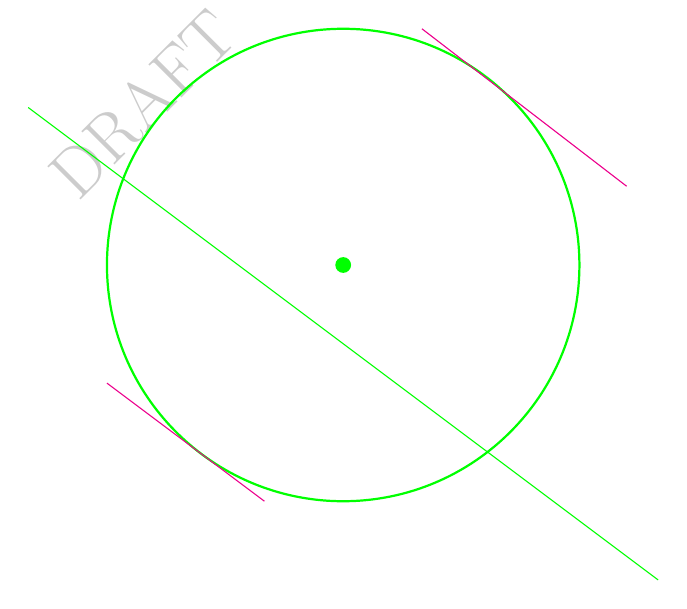
\begin{tikzpicture}[transform shape,scale=1]
		\draw[thick,green] (3,-1) circle (3);
		\fill[green] (3,-1) circle (1 mm);
		\draw[green](-1,1)--(7,-5);
		\draw[magenta](0,-2.5)--(2,-4);
		\draw[magenta](6.6,0)--(4,2);
	\end{tikzpicture}\\
	\\ 
	\textcolor{magenta}{[ঢাকা বোর্ড-২০২২]}\\
(7)	দেখাও যে, $3x-4y-5=0$ রেখাটি  $x^2+y^2-6x+8y+9=0$ বৃত্তের একটি স্পর্শক। 
	\\
	\begin{align*}
		x^2+y^2-6x+8y+9&=0\\
		\boxed{\textcolor{blue}{x^2+y^2+2gx+2fy+c=0}}&\\
		x^2+y^2+2(-3)x+2(4)y+(9)&=0
	\end{align*}
	\\
	কেন্দ্র 	$(-g,-f)=(3,-4)$ ও ব্যাসার্ধ= $\sqrt{(-3)^2+(4)^2-9}=\sqrt{9+16-9}=4$\\
	\\ 
	\textcolor{blue}{$P(x_1,y_1)$ বিন্দু হতে  $ax+by+c=0$ সরলরেখার উপর অঙ্কিত লম্বের দৈর্ঘ্য বা লম্ব দূরত্ব \\
		\\
		$d=\frac{|ax_1+by_1+c|}{\sqrt{a^2+b^2}}$}\\
	\\
	কেন্দ্র \textcolor{green}{$(3,-4)$} হতে \textcolor{magenta}{$3x-4y-5=0$}  রেখার লম্ব দূরত্ব \\
	\begin{align*}
		d=	&\frac{|3(3)-4(-4)-5|}{\sqrt{3^2+(-4)^2}}\\
		\\
		=	&	\frac{|9+16-5|}{\sqrt{25}}\\
		\\
		=	&	\frac{20}{5}\\
		\\
		=&4
	\end{align*}
	কেন্দ্র \textcolor{green}{$(3,-4)$} হতে \textcolor{magenta}{$3x-4y-5=0$}  রেখার লম্ব দূরত্ব $(4)$= বৃত্তের ব্যাসার্ধ $(4)$\\
	\\
	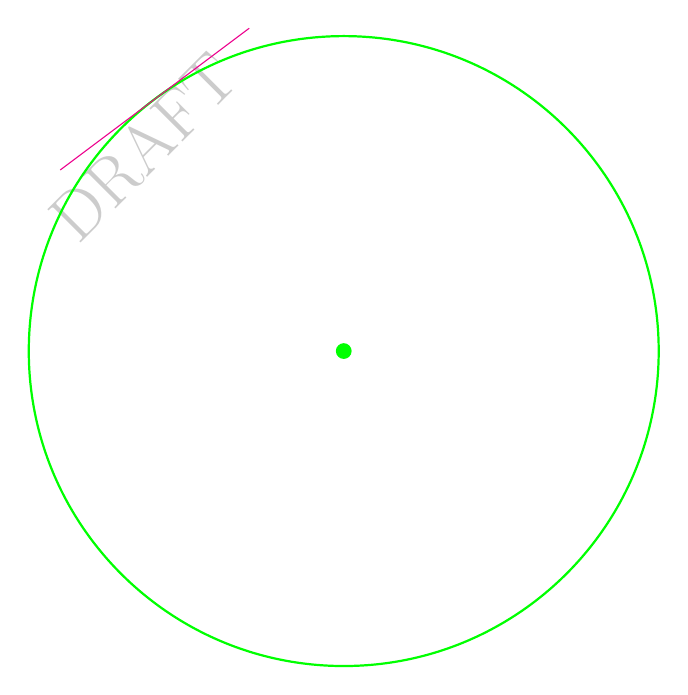
\begin{tikzpicture}[transform shape,scale=1]
	\draw[thick,green] (3,-4) circle (4);
	\fill[green] (3,-4) circle (1 mm);
	\draw[magenta](-0.6,-1.7)--(1.8,0.1);
\end{tikzpicture}\\
\\
	\textcolor{magenta}{[দিনাজপুর বোর্ড-২০১৬]}\\ 
(8)	$x^2+y^2-8x-10y-8=0$ বৃত্তের একটি স্পর্শকের সমীকরণ নির্ণয় কর যা $5x-12y=9$ এর সমান্তরাল । \\ 
	\\ 
	\textcolor{magenta}{[ঢাকা বোর্ড-২০১৯]}\\ 
(9)  $x^2+y^2-10x+6y+9=0$ বৃত্তের এরুপ দুইটি স্পর্শকের সমীকরণ নির্ণয় কর যারা   $3x+4y=2$ রেখার উপর লম্ব হবে। \\ 
	\\ 
	\begin{align*}
		x^2+y^2-10x+6y+9&=0\\
		\boxed{\textcolor{blue}{x^2+y^2+2gx+2fy+c=0}}&\\
		x^2+y^2+2(-5)x+2(3)y+(9)&=0
	\end{align*}
	\\
	কেন্দ্র 	$(-g,-f)=(5,-3)$ ও ব্যাসার্ধ= $\sqrt{(-5)^2+(3)^2-9}=\sqrt{25+9-9}=5$\\
	\\ 
	ধরি,  $3x+4y-2=0$ এর লম্ব রেখার সমীকরণ  $4x-3y+k=0$ যা বৃত্তের একটি স্পর্শক।\\
	\\  
	\textcolor{blue}{$P(x_1,y_1)$ বিন্দু হতে  $ax+by+c=0$ সরলরেখার উপর অঙ্কিত লম্বের দৈর্ঘ্য বা লম্ব দূরত্ব \\
		\\
		$\left[d=\frac{|ax_1+by_1+c|}{\sqrt{a^2+b^2}}\right]$}\\
	\\
	কেন্দ্র \textcolor{green}{$(5,-3)$} হতে স্পর্শক \textcolor{magenta}{$4x-3y+k=0$}  রেখার লম্ব দূরত্ব \\
	\begin{align*}
		d=	&\frac{|4(5)-3(-3)+k|}{\sqrt{4^2+(-3)^2}}\\
		\\
		=	&	\frac{|20+9+k|}{\sqrt{25}}\\
		\\
		=	&	\frac{|k+29|}{5}\\
	\end{align*}
	আমরা জানি, বৃত্তের কেন্দ্র হতে স্পর্শকের লম্ব দূরত্ব বৃত্তের ব্যাসার্ধের সমান। \\
	\\ 
	\begin{align*}
		\frac{|k+29|}{5}&=5\\
		\\
		\pm (k+29)&=25\\
		\\
		k+29&=\pm 25\\
		\\
		k&=\pm 25-29\\
		\\
		k&=+25-29,\,\,\,-25-29\\
		\\
		k&=-4,\,\,\,-54
	\end{align*}
	\\
	$4x-3y+k=0$ সমীকরণে $k$ এর মান বসিয়ে পাই \\ 
	বৃত্তের স্পর্শক \\ 
	$4x-3y-4=0$\\
	\\
	$4x-3y-54=0$\\
	\\
উপরোক্ত স্পর্শকের সমীকরণগুলি $3x+4y=2$ রেখার উপর লম্ব হবে। \\ 
		\begin{tikzpicture}[transform shape,scale=1]
		\draw[thick,green] (5,-3) circle (5);
		\fill[green] (5,-3) circle (1 mm);
		\draw[green](-2,2)--(14,-10);
			\draw[magenta](4,4)--(-2,-4);
			\draw[magenta](6,-10)--(15,2);	
	\end{tikzpicture}\\
\\ 
	\textcolor{magenta}{[ঢাকা বোর্ড-২০১৬]}\\ 
	(10) $x^2+y^2-2x-4y-4=0$ বৃত্তের স্পর্শক  $3x-4y+5=0$ রেখার উপর লম্ব হলে স্পর্শকের সমীকরণ নির্ণয় কর ।  \\ 
	\\ 
	\textcolor{magenta}{[দিনাজপুর বোর্ড-২০১৪]}\\ 
(11)	$x^2+y^2+4x-8y+2=0$ বৃত্তের স্পর্শক অক্ষদ্বয় হতে একই চিহ্ন বিশিষ্ট সমমানের অংশ ছেদ করে। স্পর্শকের সমীকরণ নির্ণয় কর।   \\
	\begin{align*}
		x^2+y^2+4x-8y+2&=0\\
		\boxed{\textcolor{blue}{x^2+y^2+2gx+2fy+c=0}}&\\
		x^2+y^2+2(2)x+2(-4)y+(2)&=0
	\end{align*}
	\\
	কেন্দ্র 	$(-g,-f)=(-2,4)$ ও ব্যাসার্ধ= $\sqrt{(2)^2+(-4)^2-2}=\sqrt{4+16-2}=3\sqrt{2}$\\
	\\  
	\\
	\textcolor{blue}{ দ্বি খণ্ডন আকার  Two	Intercept form}\\
	\\
	$\textcolor{blue}{\frac{x}{a}+\frac{y}{b}=1}$\\
	\\
	স্পর্শক অক্ষদ্বয় হতে একই চিহ্ন বিশিষ্ট সমমানের অংশ ছেদ করে. $a=b$\\
	\\
	\begin{align*}
		\frac{x}{a}+\frac{y}{b}&=1\\
		\\
		\frac{x}{a}+\frac{y}{a}&=1\\
		\\
		x+y&=a\\
		\\
		x+y-a&=0
	\end{align*}
	\\  
	\textcolor{blue}{$P(x_1,y_1)$ বিন্দু হতে  $ax+by+c=0$ সরলরেখার উপর অঙ্কিত লম্বের দৈর্ঘ্য বা লম্ব দূরত্ব \\
		\\
		$\left[d=\frac{|ax_1+by_1+c|}{\sqrt{a^2+b^2}}\right]$}\\
	\\
	কেন্দ্র \textcolor{green}{$(-2,4)$} হতে স্পর্শক \textcolor{magenta}{$x+y-a=0$}  রেখার লম্ব দূরত্ব \\
	\begin{align*}
		d=	&\frac{|(-2)+(4)-a|}{\sqrt{1^2+1^2}}\\
		\\
		=	&	\frac{|2-a|}{\sqrt{2}}\\
	\end{align*}
	আমরা জানি, বৃত্তের কেন্দ্র হতে স্পর্শকের লম্ব দূরত্ব বৃত্তের ব্যাসার্ধের সমান। \\
	\\ 
	\begin{align*}
		\frac{|2-a|}{\sqrt{2}}&=3\sqrt{2}\\
		\\
		|2-a|&=3\sqrt{2}\,\,\sqrt{2}\\
		\\
		2-a&=\pm 6\\
		\\
		a&=2\pm 6-2\\
		\\
		a&=2+6,\,\,\,2-6\\
		\\
		a&=8,\,\,\,-4
	\end{align*}
	\\
	$x+y-a=0$ সমীকরণে $a$ এর মান বসিয়ে পাই\\ 
	বৃত্তের স্পর্শক \\ 
	$x+y-8=0$\\
	\\
	$x+y+4=0$\\
স্পর্শকগুলি অক্ষদ্বয় হতে একই চিহ্ন বিশিষ্ট সমমানের অংশ ছেদ করে। 
		\\
	\begin{tikzpicture}[transform shape,scale=1]
			\draw [-latex,thick,red](-10,0) -- (10,0) node[right] {$x$} coordinate(x axis);
		\draw [-latex,thick,red](0,-10) -- (0,10) node[above] {$y$} coordinate(y axis);
		\draw[thick,green] (-2,4) circle (4.24);
		\fill[green] (-2,4) circle (1 mm);
		\draw[magenta](-8,4)--(2,-6);
			\draw[magenta](10,-2)--(-2,10);
	\end{tikzpicture}\\
	\\
	\textcolor{magenta}{[RUET-09-10]}\\
(12)	$x^2+y^2+4x-8y+2=0$ বৃত্তটির এমন স্পর্শকগুলির সমীকরণ নির্ণয় কর যারা অক্ষদ্বয়কে সমান ও বিপরীত চিহ্নে খন্ডিত করে। \\
	\begin{align*}
		x^2+y^2+4x-8y+2&=0\\
		\boxed{\textcolor{blue}{x^2+y^2+2gx+2fy+c=0}}&\\
		x^2+y^2+2(2)x+2(-4)y+(2)&=0
	\end{align*}
	\\
	কেন্দ্র 	$(-g,-f)=(-2,4)$ ও ব্যাসার্ধ= $\sqrt{2^2+(-4)^2-2}=\sqrt{4+16-2}=3\sqrt{2}$\\
	\\  
	\\
	\textcolor{blue}{ দ্বি খণ্ডন আকার  Two	Intercept form}\\
	\\
	$\textcolor{blue}{\frac{x}{a}+\frac{y}{b}=1}$\\
	\\
	স্পর্শক অক্ষদ্বয়কে সমান এবং বিপরীত চিহ্নে খন্ডিত করে. $b=-a$\\
	\\
	\begin{align*}
		\frac{x}{a}+\frac{y}{b}&=1\\
		\\
		\frac{x}{a}+\frac{y}{-a}&=1\\
		\\
		x-y&=a\\
		\\
		x-y-a&=0
	\end{align*}
	\\  
	\textcolor{blue}{$P(x_1,y_1)$ বিন্দু হতে  $ax+by+c=0$ সরলরেখার উপর অঙ্কিত লম্বের দৈর্ঘ্য বা লম্ব দূরত্ব \\
		\\
		$\left[d=\frac{|ax_1+by_1+c|}{\sqrt{a^2+b^2}}\right]$}\\
	\\
	কেন্দ্র \textcolor{green}{$(-2,4)$} হতে স্পর্শক \textcolor{magenta}{$x-y-a=0$}  রেখার লম্ব দূরত্ব \\
	\begin{align*}
		d=	&\frac{|(-2)-(4)-a|}{\sqrt{1^2+1^2}}\\
		\\
		=	&	\frac{|-6-a|}{\sqrt{2}}\\
	\end{align*}
	আমরা জানি, বৃত্তের কেন্দ্র হতে স্পর্শকের লম্ব দূরত্ব বৃত্তের ব্যাসার্ধের সমান। \\
	\\ 
	\begin{align*}
		\frac{|-6-a|}{\sqrt{2}}&=3\sqrt{2}\\
		\\
		|a+6|&=3\sqrt{2}\,\,\sqrt{2}\\
		\\
		a+6&=\pm 6\\
		\\
		a&=\pm 6-6\\
		\\
		a&=6-6,\,\,\,-6-6\\
		\\
		a&=0,\,\,\,-12
	\end{align*}
	\\
	$x-y-a=0$ সমীকরণে  $a$ এর মান বসিয়ে পাই\\  
	বৃত্তের স্পর্শক \\ 
	$x-y=0$ (মূল বিন্দুগামী হওয়ার কারণে গ্রহণ যোগ্য নয়)\\
	\\
	$x-y+12=0$ স্পর্শকটি অক্ষদ্বয়কে সমান ও বিপরীত চিহ্নে খন্ডিত করে। \\ 
	\\
\begin{tikzpicture}[transform shape,scale=1]
	\draw [-latex,thick,red](-13,0) -- (3,0) node[right] {$x$} coordinate(x axis);
	\draw [-latex,thick,red](0,-1) -- (0,13) node[above] {$y$} coordinate(y axis);
	\draw[thick,green] (-2,4) circle (4.24);
	\fill[green] (-2,4) circle (1 mm);
	\draw[magenta](-12,0)--(0,12);
	\draw[magenta](3,3)--(-1,-1);
\end{tikzpicture}\\
\\
	\textcolor{magenta}{[সিলেট বোর্ড-২০১৪]}\\
(13)	$k$ এর মান কত হলে  $3x+4y=k$ রেখাটি $x^2+y^2=10x$ বৃত্তকে স্পর্শ করবে। \\
	\begin{align*}
		x^2+y^2&=10x\\
		\\
		x^2+y^2-10x&=0\\
		\boxed{\textcolor{blue}{x^2+y^2+2gx+2fy+c=0}}&\\
		x^2+y^2+2(-5)x+2(0)y+(0)&=0
	\end{align*}
	\\
	কেন্দ্র 	$(-g,-f)=(5,0)$ ও ব্যাসার্ধ= $\sqrt{(-5)^2+(0)^2-0}=\sqrt{25}=5$\\
	\\  
	\textcolor{blue}{$P(x_1,y_1)$ বিন্দু হতে  $ax+by+c=0$ সরলরেখার উপর অঙ্কিত লম্বের দৈর্ঘ্য বা লম্ব দূরত্ব \\
		\\
		$\left[d=\frac{|ax_1+by_1+c|}{\sqrt{a^2+b^2}}\right]$}\\
	\\
	কেন্দ্র \textcolor{green}{$(5,0)$} হতে স্পর্শক \textcolor{magenta}{$3x+4y-k=0$}  রেখার লম্ব দূরত্ব \\
	\begin{align*}
		d=	&\frac{|3(5)+4(0)-k|}{\sqrt{3^2+4^2}}\\
		\\
		=	&	\frac{|15-k|}{\sqrt{25}}\\
		\\
		=	&	\frac{|15-k|}{5}\\
	\end{align*}
	আমরা জানি, বৃত্তের কেন্দ্র হতে স্পর্শকের লম্ব দূরত্ব বৃত্তের ব্যাসার্ধের সমান। \\
	\\ 
	\begin{align*}
		\frac{|15-k|}{5}&=5\\
		\\
		\pm (15-k)&=25\\
		\\
		15-k&=\pm 25\\
		\\
		k&=15\pm 25\\
		\\
		k&=15+25,\,\,\,15-25\\
		\\
		k&=40,\,\,\,-10
	\end{align*}
	\\ 
	\textcolor{magenta}{[কুমিল্লা বোর্ড-২০১২]}\\
(14)	$x^2+y^2-8x-2y+4=0$ বৃত্তের একটি স্পর্শক  $3x+by-1=0$ হলে  $b$ এর মান নির্ণয় কর\\
	\\
	\begin{align*}
		x^2+y^2-8x-2y+4&=0\\
		\boxed{\textcolor{blue}{x^2+y^2+2gx+2fy+c=0}}&\\
		x^2+y^2+2(-4)x+2(-1)y+(4)&=0
	\end{align*}
	\\
	কেন্দ্র 	$(-g,-f)=(4,1)$ ও ব্যাসার্ধ= $\sqrt{(-4)^2+(-1)^2-4}=\sqrt{16+1-4}=\sqrt{13}$\\
	\\   
	\textcolor{blue}{$P(x_1,y_1)$ বিন্দু হতে  $ax+by+c=0$ সরলরেখার উপর অঙ্কিত লম্বের দৈর্ঘ্য বা লম্ব দূরত্ব \\
		\\
		$\left[d=\frac{|ax_1+by_1+c|}{\sqrt{a^2+b^2}}\right]$}\\
	\\
	কেন্দ্র \textcolor{green}{$(4,1)$} হতে স্পর্শক \textcolor{magenta}{$3x+by-1=0$}  রেখার লম্ব দূরত্ব \\
	\begin{align*}
		d=	&\frac{|3(4)+b(1)-1|}{\sqrt{3^2+b^2}}\\
		\\
		=	&	\frac{|12+b-1|}{\sqrt{b^2+9}}\\
		\\
		=	&	\frac{|11+b|}{\sqrt{b^2+9}}\\
	\end{align*}
	আমরা জানি, বৃত্তের কেন্দ্র হতে স্পর্শকের লম্ব দূরত্ব বৃত্তের ব্যাসার্ধের সমান। \\
	\\ 
	\begin{align*}
		\frac{|11+b|}{\sqrt{b^2+9}}&=\sqrt{13}\\
		\\
		|b+11|&=\sqrt{13}\,\,\,\sqrt{b^2+9}\\
		\\
		(b+11)^2&= (13)(b^2+9)\\
		\\
		b^2+22b+121&=13b^2+117\\
		\\
		12b^2-22b-4&=0\\
		\\
		6b^2-11b-2&=0\\
		\\
		6b^2-12b+b-2&=0\\
		\\
		6b(b-2)+1(b-2)&=0\\
		\\
		(b-2)(6b+1)&=0\\
		\\
		b=&2,\,\,\,-\frac{1}{6}
	\end{align*}
	\\ 
	\textcolor{magenta}{[চট্রগ্রাম বোর্ড-২০১৪]}\\
(15)	দেখাও যে, $lx+my=1$ রেখাটি $x^2+y^2-2ax=0$ বৃত্তকে স্পর্শ করবে যদি $a^2m^2+2al=1$ হয়\\
	\begin{align*}
		x^2+y^2-2ax&=0\\
		\boxed{\textcolor{blue}{x^2+y^2+2gx+2fy+c=0}}&\\
		x^2+y^2+2(-a)x+2(0)y+(0)&=0
	\end{align*}
	\\
	কেন্দ্র 	$(-g,-f)=(a,0)$ ও ব্যাসার্ধ= $\sqrt{(-a)^2+(0)^2-0}=\sqrt{a^2}=a$\\
	\\   
	\textcolor{blue}{$P(x_1,y_1)$ বিন্দু হতে  $ax+by+c=0$ সরলরেখার উপর অঙ্কিত লম্বের দৈর্ঘ্য বা লম্ব দূরত্ব \\
		\\
		$\left[d=\frac{|ax_1+by_1+c|}{\sqrt{a^2+b^2}}\right]$}\\
	\\
	কেন্দ্র \textcolor{green}{$(a,0)$} হতে স্পর্শক \textcolor{magenta}{$lx+my-1=0$}  রেখার লম্ব দূরত্ব \\
	\begin{align*}
		d=	&\frac{|l(a)+m(0)-1|}{\sqrt{l^2+m^2}}\\
		\\
		=	&	\frac{|al-1|}{\sqrt{l^2+m^2}}\\
		\\
		=	&	\frac{|al-1|}{\sqrt{l^2+m^2}}\\
	\end{align*}
	আমরা জানি, বৃত্তের কেন্দ্র হতে স্পর্শকের লম্ব দূরত্ব বৃত্তের ব্যাসার্ধের সমান। \\
	\\ 
	\begin{align*}
		\frac{|al-1|}{\sqrt{l^2+m^2}}&=a\\
		\\
		|al-1|&=a\,\,\,\sqrt{l^2+m^2}\\
		\\
		(al-1)^2&= a^2\,\,(l^2+m^2)\\
		\\
		a^2\,l^2-2\,a\,l+1&=a^2\,l^2+a^2\,m^2\\
		\\
		a^2\,m^2+2\,a\,l&=1\\
	\end{align*}
	\\ 
	\textcolor{magenta}{[যশোর বোর্ড-২০১২]}\\
(16)	$px+qy=1$ রেখাটি $x^2+y^2=a^2$ বৃত্তকে স্পর্শ করে। দেখাও যে,  $(p,q)$ বিন্দুটি একটি বৃত্তের উপর অবস্থিত। \\
	\begin{align*}
		x^2+y^2&=a^2\\
	\end{align*}
	\\
	কেন্দ্র 	$(0,0)$ ও ব্যাসার্ধ= $a$\\
	\\   
	\textcolor{blue}{$P(x_1,y_1)$ বিন্দু হতে  $ax+by+c=0$ সরলরেখার উপর অঙ্কিত লম্বের দৈর্ঘ্য বা লম্ব দূরত্ব \\
		\\
		$\left[d=\frac{|ax_1+by_1+c|}{\sqrt{a^2+b^2}}\right]$}\\
	\\
	কেন্দ্র \textcolor{green}{$(0,0)$} হতে স্পর্শক \textcolor{magenta}{$px+qy-1=0$}  রেখার লম্ব দূরত্ব \\
	\begin{align*}
		d=	&\frac{|p(0)+q(0)-1|}{\sqrt{p^2+q^2}}\\
		\\
		=	&	\frac{|-1|}{\sqrt{p^2+q^2}}\\
		\\
		=	&	\frac{1}{\sqrt{p^2+q^2}}\\
	\end{align*}
	আমরা জানি, বৃত্তের কেন্দ্র হতে স্পর্শকের লম্ব দূরত্ব বৃত্তের ব্যাসার্ধের সমান। \\
	\\ 
	\begin{align*}
		\frac{1}{\sqrt{p^2+q^2}}&=a\\
		\\
		\frac{1}{p^2+q^2}&=a^2\\
		\\
		p^2+q^2&= \frac{1}{a^2}\\
	\end{align*}
	\\ 
	$(p,q)$ বিন্দুটি  $x^2+y^2=\frac{1}{a^2}$ সমীকরণ দ্বারা নির্দেশিত বৃত্তের উপর অবস্থিত।\\
\end{document}